\documentclass[12pt,a4paper,titlepage]{scrreprt}
\usepackage[utf8]{inputenc}
\usepackage[english]{babel}

\usepackage[backend=biber,style=alphabetic,natbib=true]{biblatex}
\usepackage{url}
\usepackage{hyperref}
\usepackage{fancyvrb}
\usepackage{csquotes}
\usepackage{upquote}

\usepackage{amsmath}
\usepackage{amssymb}

\newcommand{\catC}{\mathbb{C}}
\newcommand{\catD}{\mathbb{D}}
\newcommand{\opcat}[1]{{#1}^{\text{op}}}
\newcommand{\Sets}{\mathbf{Sets}}

%% @TODO: invent some kid of inline 'code' style for this
\newcommand{\firstArr}{\texttt{first}}

\DefineVerbatimEnvironment{code}{Verbatim}{fontsize=\small}

\hypersetup{
    colorlinks,
    linkcolor=black,
    citecolor=black,
    filecolor=black,
    urlcolor=black
}

\bibliography{literature}

\title{Cat-arrows}
\author{%
    Johannes Emerich
        (\href{mailto:Johannes@emerich.de}{johannes@emerich.de})\\
    Ignas Vyšniauskas
        (\href{mailto:i.vysniauskas@gmail.com}{i.vysniauskas@gmail.com})
}
\date{}

\begin{document}


\maketitle

\begin{abstract}
    This is a report on Arrows.
\end{abstract}

\section{Context}
\begin{frame}
\frametitle{Liberating Programming from the ``von Neumann'' style}

\begin{itemize}
    \item John Backus' call for new language paradigm (1978)
    \begin{itemize}
        \item \emph{Functional} programming (``FP'') as combinatorial
              approach to program construction
        \item Construct programs in an algebra of programs
        \item Variables range over \emph{programs}, operations are \emph{on}
              programs (\emph{pointfree} style)
        \item Functional style: only one state transition per operation
    \end{itemize}
    \item Haskell as most popular language true to Backus' ideas
\end{itemize}
\end{frame}

\begin{frame}
\frametitle{Haskell is non-strict}

\begin{columns}[c]
    \begin{column}{.6\textwidth}
        \begin{itemize}
            \item Problem of functions in computing: non-termination
            \item \emph{Lift} all types by adding an \texttt{undefined} ($\bot$) bottom
                  element, lowest in information order
            \item Set $B = \{\textrm{True}, \textrm{False}\}$ lifted to $B_\bot
                  = B \cup \{\bot\}$
            \item Functions are $B_\bot \to B_\bot$
        \end{itemize}
    \end{column}
    \begin{column}{.4\textwidth}
        \begin{center}
        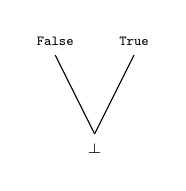
\begin{tikzpicture}
            \draw[font=\tiny] (0,0) node[below] {$\bot$} -- (0.5,1) node[above] {\texttt{True}};
            \draw[font=\tiny] (0,0) -- (-0.5,1) node[above] {\texttt{False}};
        \end{tikzpicture}
        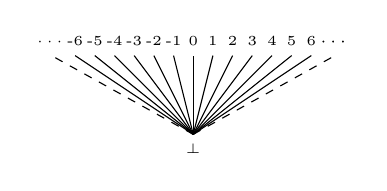
\begin{tikzpicture}
            \draw[dashed, font=\tiny] (0,0) -- (1.8,1) node[above] {$\cdots$};
            \draw[font=\tiny] (1.8,1) node[above] {$\cdots$};
            \draw[font=\tiny] (0,0) -- (1.5,1) node[above] {6};
            \draw[font=\tiny] (0,0) -- (1.25,1) node[above] {5};
            \draw[font=\tiny] (0,0) -- (1.0,1) node[above] {4};
            \draw[font=\tiny] (0,0) -- (0.75,1) node[above] {3};
            \draw[font=\tiny] (0,0) -- (0.5,1) node[above] {2};
            \draw[font=\tiny] (0,0) -- (0.25,1) node[above] {1};
            \draw[font=\tiny] (0,0) node[below] {$\bot$} -- (0,1) node[above] {0};
            \draw[font=\tiny] (0,0) -- (-0.25,1) node[above] {-1};
            \draw[font=\tiny] (0,0) -- (-0.5,1) node[above] {-2};
            \draw[font=\tiny] (0,0) -- (-0.75,1) node[above] {-3};
            \draw[font=\tiny] (0,0) -- (-1,1) node[above] {-4};
            \draw[font=\tiny] (0,0) -- (-1.25,1) node[above] {-5};
            \draw[font=\tiny] (0,0) -- (-1.5,1) node[above] {-6};
            \draw[dashed, font=\tiny] (0,0) -- (-1.8,1) node[above] {$\cdots$};
        \end{tikzpicture}
        \end{center}
    \end{column}
\end{columns}
\end{frame}

\begin{frame}[fragile]
\frametitle{Haskell is non-strict}
\begin{itemize}
    \item \emph{Strict} semantics
          \[
            \forall f: A_\bot \to B_\bot, f(\bot) = \bot
          \]
    \item Non-strict semantics allow operating on (potentially) infinite data
          structures:
          \begin{center}\verb|or ([True] ++ repeat False) == True|\end{center}
    \item Expressions only partially evaluated (\emph{thunks}) until value needed
    \item Problem for effectful computations whose result is never
          needed, e.g.
          \begin{center}\verb|print "Hello, Dave!"|\end{center}
\end{itemize}
\end{frame}

\begin{frame}[fragile]
\frametitle{Haskell is pure}
\begin{itemize}
    \item Functions are mappings from domain to codomain
    \item Haskell functions are \emph{pure}, they are \emph{only} mappings
    \item No side-effects (input/output, changes to global state)
    \item Beneficial for achieving Backus' desiderata
    \item But side-effects are desirable feature of programs
    \item How to bring them back in?
\end{itemize}
\end{frame}

\begin{frame}[fragile]
\frametitle{Computational lambda-calculus and monads}
\begin{itemize}
    \item Eugenio Moggi ('89): program equivalence in $\lambda$-calculus
    \item Semantics for \emph{general} notion of computation
          \begin{itemize}
              \item Side-effects, non-determinism, non-termination
          \end{itemize}
    \item Categorical language semantics with types as objects
          \begin{itemize}
              \item Distinguish type $B$ from corresponding \emph{computations} $TB$
              \item Model each notion of computation as a monad
          \end{itemize}
    \item Adopted into Haskell as general interface to computation
          \begin{itemize}
              \item Functions have to be pure, computations don't
          \end{itemize}
\end{itemize}
\end{frame}

\section{A short history of the categorical aspects of arrows}
\label{sec:cat-arrows-hist}

Unlike Monads, which were borrowed from category theory to model various
computational behaviours, arrows were at first introduced by
Hughes~\cite{hughes-monad2arr} purely as a computational concept. Hence
categorical \emph{interpretations} of arrows came only as an afterthought.
Unsurprisingly, a whole family of interpretations was thus born, which we try
to describe briefly here. % and possibly expand on it later on

The tale of the categorical semantics of arrows begins with a folklore
statement
\begin{displayquote}Arrows are Freyd categories.\end{displayquote}
%% wtf -- this quoting is ugly -- want emph + quotemarks @TODO: fix
which is perhaps first noted by Paterson~\cite{paterson}.

This statement was first verified in detail by Heunen and
Jacobs~\cite{arr-like-mon}. Since computationally arrows are a generalisation
of monads, it is perhaps not so surprising that the situation turns out to be
similar categorically. Namely, Heunen and Jacobs prove that arrows can be
seen as monoids in categories of bifunctors $\opcat{\catC} \times \catC \to
\catC$, just like monads are monoids in a category of endofunctors.
Furthermore, they show there is a bijective correspondence between locally
small Freyd categories $\catC \to \catD$ and arrows over $\catC$.

However, the construction is slightly flawed due to issues with the size of
$\catC$.\footnote{$\catC$ would need to be both small and (co)complete, however
this is impossible~\cite[Chapter 3]{freyd-abelian-cats}} %% @TODO: insert citation
Hence, the statement \enquote{Arrows are Freyd} is only proved for bifunctors
on $\opcat{\catC} \times \catC \to \Sets$, where $\catC$ is \emph{small} (i.e.\ 
profunctors) with an assumption that it would be possible to achieve the same
result in an enriched setting.

A later paper by Hasuo and Jacobs called ``Freyd is Kleisli, for
Arrows''~\cite{freyd-is-kleisli} elaborates on the fact that the correspondence
is actually an instance of the well-known Kleisli construction for monads,
adapted for arrows. This again goes along with the general intuition that
arrows are a generalisation of monads.

%% @TODO: I'm not sure whether my interpretation of this is fully correct.
%% In particular, I need to check whether they are just examining the same
%% correspondance, or building something new.
%% They seem to be talking about a 'monoidal' interpretation and a Freyd one,
%% as of two different things...
%% Perhaps it's best to re-iterate this statement after we write-up the
%% 'meat' parts.

Another paper by Jacobs, Heunen and Hasuo~\cite{cat-semantics-arr} combines the
previous results into a self-contained paper and will be our primary reference.

Finally, a paper by Atkey~\cite{atkey-fix} notes that the work of Jacobs et.~al
slightly misinterprets the situation. Firstly, Atkey elaborates on the fact
that it is necessary to consider enriched Freyd categories, because in order to
provide denotational semantics for arrows one needs to consider a \emph{type}
of morphisms between objects (which are types too), hence one needs at least
some sort of self-enrichment. More importantly, Atkey observes that the
\firstArr{} operator allows arrows to take \emph{unstructured} input. This does
not fit-in with the simplified ``Arrows are Freyd'' view, because it implies
that all computations are structured, which prevents modelling unstructured
input. Atkey thus shows that one also needs to consider indexed Freyd categories and
proves various relations between \{closed, indexed, enriched\} Freyd categories,
arrows and strong monads.


\printbibliography

\end{document}
